\section{vLLM Performance Dashboard}
{{\footnotesize
\begin{description}[labelwidth=5em, labelsep=1em, leftmargin=*, align=left, itemsep=0.3em, parsep=0em]
  \item[date:] 2022-06-22
  \item[last\_updated:] 2025-01
  \item[expired:] unkown
  \item[valid:] yes
  \item[url:] \href{https://simon-mo-workspace.observablehq.cloud/vllm-dashboard-v0/}{https://simon-mo-workspace.observablehq.cloud/vllm-dashboard-v0/}
  \item[domain:] LLM; HPC/inference
  \item[focus:] Interactive dashboard showing inference performance of vLLM
  \item[keywords:]
    - Dashboard
    - Throughput visualization
    - Latency analysis
    - Metric tracking
  \item[task\_types:]
    - Performance visualization
  \item[ai\_capability\_measured:]
    - Throughput
    - latency
    - hardware utilization
  \item[metrics:]
    - Tokens/sec
    - TTFT
    - Memory usage
  \item[models:]
    - LLaMA-2
    - Mistral
    - Qwen
  \item[ml\_motif:]
    - HPC/inference
  \item[type:] Framework
  \item[ml\_task:] Visualization
  \item[notes:] Built using ObservableHQ; integrates live data from vLLM benchmarks.
  \item[contact.name:] Simon Mo
  \item[contact.email:] unkown
  \item[results.name:] ChatGPT LLM
  \item[results.url:] \href{unkown}{unkown}
  \item[fair.reproducible:] Yes
  \item[fair.benchmark\_ready:] Yes
  \item[ratings.software.rating:] 0
  \item[ratings.software.reason:] Not analyzed.
  \item[ratings.specification.rating:] 8.0
  \item[ratings.specification.reason:] Framed as a model-serving tool rather than a benchmark, but includes benchmark configurations and real model tasks.
  \item[ratings.dataset.rating:] 6.0
  \item[ratings.dataset.reason:] Mostly uses dummy configs or external model endpoints for evaluation; not designed around a formal dataset.
  \item[ratings.metrics.rating:] 8.0
  \item[ratings.metrics.reason:] Well-defined serving metrics: tokens/sec, time-to-first-token, and gain over baselines.
  \item[ratings.reference\_solution.rating:] 9.0
  \item[ratings.reference\_solution.reason:] Core framework includes full reproducible serving benchmarks and code; multiple deployment case studies.
  \item[ratings.documentation.rating:] 9.0
  \item[ratings.documentation.reason:] High-quality usage guides, examples, and performance tuning docs.
  \item[id:] vllm\_performance\_dashboard
  \item[Citations:] \cite{mo2024vllm_dashboard}
  \item[Ratings:]
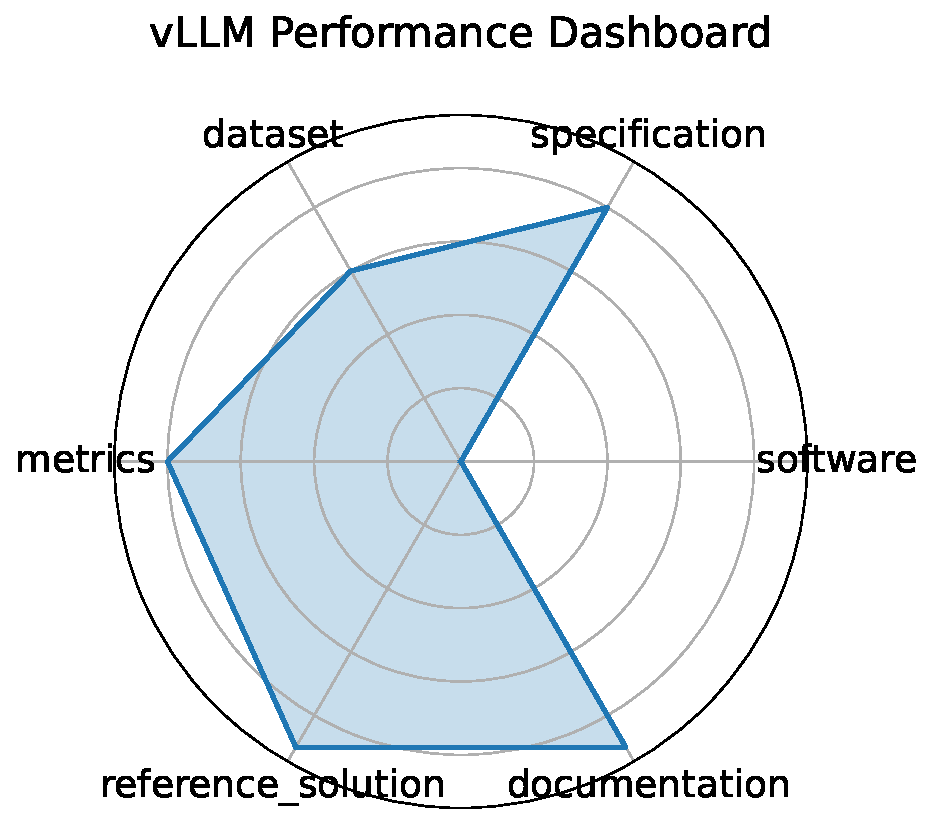
\includegraphics[width=0.2\textwidth]{vllm_performance_dashboard_radar.pdf}
\end{description}
}}
\clearpage